\chapter{Results and Analysis}

We performed classification with four different classifiers on four different datasets. In each dataset-classifier combination we measured classification accuracy when applying four different feature selection (FS) methods. The aim is to investigate the impact of feature selection on classification accuracy, and the interaction between different classifiers and FS-methods. To enable a basis for comparisons, classification accuracy was measured without FS too.

\section{Impact of Factors: Datasets, Classifiers and FS-methods}
\label{Variation_among_factors}

Before analyzing the results we consider potential interactions between different factors involved in the experiment, these are:

\begin{enumerate}
  \item Datasets
  \item Machine Learning classifiers
  \item Feature selection methods
\end{enumerate}

Having four of each factor, there are 16 distinct combinations of classifiers and FS-methods with four measurements, one on each dataset. All datasets contain different information and therefore introduce necessary variance to the experiments. The variance allows us to suspect these results generalizes well onto other datasets in the domain of breast cancer, which are not included in this study. In our scope we are particular interested in the interaction of classifiers and FS-methods.

% \begin{figure*}[ht]
  \centering
    \begin{subfigure}[b]{0.475\textwidth}
        \centering
        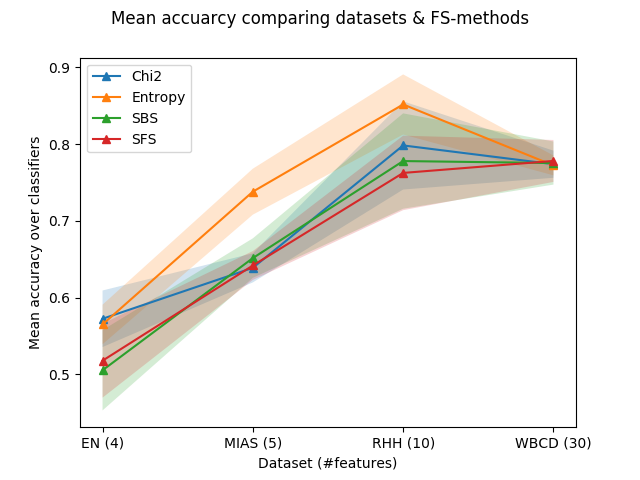
\includegraphics[width=\textwidth]{../plots_with_std_fill/comp_acc_datasets.png}
        \caption[]%
        {{\small Datasets and accuracy displays evident correlation independently of applied FS method.}}
        \label{fig:comp_acc_datasets}
    \end{subfigure}
  \hfill
    \begin{subfigure}[b]{0.475\textwidth}
        \centering
        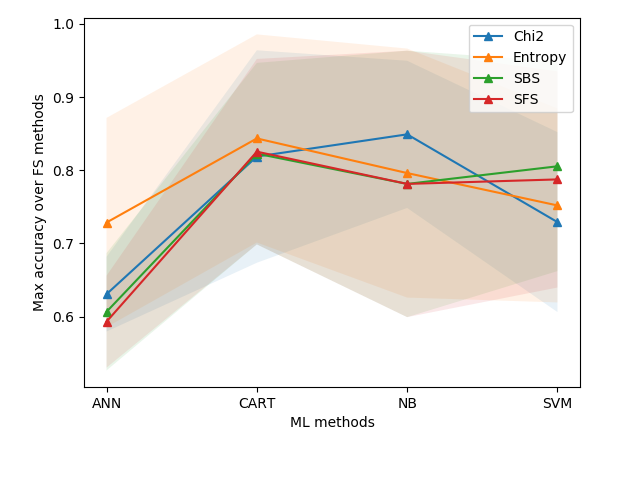
\includegraphics[width=\textwidth]{../plots_with_std_fill/comp_classif_datasets.png}
        \caption[]%
        {{\small Some correlation between different classifiers and FS-methods is evident.}}
        \label{fig:comp_classif_datasets}
    \end{subfigure}
  \caption[]
  {\small Good caption goes here.}
  \label{fig:anova_plots}
\end{figure*}


\subsection{Evaluation of FS-methods and Classifiers}
\label{sec:fs_methods_classifiers}

To investigate the effect of feature selection on different classifiers, we performed two-way ANOVA. The values constitutes of each accuracy achieved by all distinct classifier and FS-method combinations, on all datasets. The ANOVA result is presented in table \ref{table:anova_values_classif}.

\begin{table}[ht]
  \begin{center}
  \begin{tabular}{l|r|r|r|r|r|r|}
  \cline{2-7}
  & $RSS$ & $df$ & $F$ & $P(>F)$ & $\eta^2$ & $\omega^2$ \\ \cline{1-7}
  \multicolumn{1}{ |l| }{\textbf{Classifier}}
  & 0.3336 &  3.0 & 16.491 & 1.6860e-07 & 0.2149 & 0.2010 \\
  \cline{1-7}
  \multicolumn{1}{ |l| }{\textbf{Method}}
  & 0.7383 &  3.0 & 36.495 & 1.9503e-12 & 0.4757 & 0.4607 \\
  \cline{1-7}
  \multicolumn{1}{ |l| }{\textbf{Classifier*Method}}
  & 0.1565 &  9.0 & 2.5783 & 1.6490e-02 & 0.1008 & 0.0614 \\
  \cline{1-7}
  \multicolumn{1}{ |l| }{\textbf{Residual}}
  & 0.3237 &  48.0 \\ \cline{1-3}
  \end{tabular}
  \caption{Set caption.}
  \label{table:anova_values_classif}
  \end{center}
\end{table}


The **-significance of Classifier concludes that the selection of classifier effect what accuracy is achieved. The variance of the each respective classifier is visualized in figure \ref{fig:box_plots}. The box-plot entail that ANN on average perform worse than other classifiers. NB has the largest variance, with accuracy ranging from roughly 50\% to 100\%. CART performs the best, with the highest average accuracy.

The ANOVA result of Method conclude the selection of FS-method do not result in a significant difference in achieved accuracy. In figure \ref{fig:box_methods} all methods manifests a large variance but roughly in the same range, which emphasizes the result of the ANOVA. That is, there is no significant difference in accuracy when applying different FS-methods.

Analyzing these results together, first they suggest that the selection of classifier impacts the expected accuracy. Secondly, which FS-method is used together with the classifier do not effect expected accuracy. Lastly, no unique combination of classifier and FS-method are statistically superior to others.

It's important to note these measurements only include classification with FS-selection, they do not enable any conclusions regarding the impact of using, versus not using feature selection. Therefore, that is the next point of interest.

\begin{figure*}[ht]
  \centering
    \begin{subfigure}[b]{0.49\textwidth}
        \centering
        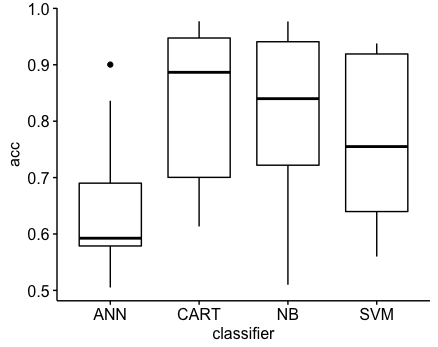
\includegraphics[width=\textwidth]{Rplots/boxplot_classifiers.png}
        \caption[]%
        {{\small}}
        \label{fig:box_classifers}
    \end{subfigure}
  \hfill
    \begin{subfigure}[b]{0.49\textwidth}
        \centering
        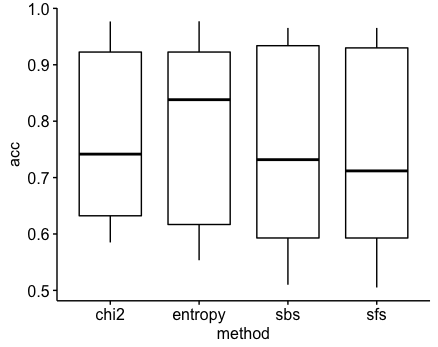
\includegraphics[width=\textwidth]{Rplots/boxplot_methods.png}
        \caption[]%
        {{\small}}
        \label{fig:box_methods}
    \end{subfigure}
  \caption[]
  {\small Variation in accuracy in respect to (a) classifiers and (b) FS-methods. Vertical axis represents accuracy. The horizontal bar in each box represents the mean accuracy. The box represents the range where 50\% of the measurements was found. The vertical lines connected to the boxes includes represents the remaining 25\% on each side. Dots represents outliers.}
  \label{fig:box_plots}
\end{figure*}


\FloatBarrier
\section{Classification Improvements}

After performing classification with and without FS-methods, all results of each classifier was collected. Results are presented in tables for ANN \ref{table:ANN}, CART \ref{table:CART}, NB \ref{table:NB} and SVM \ref{table:SVM} where the highest achieved accuracy is highlighted in bold format. The improvement is measured in gain, the ratio between best achieved FS accuracy and full dataset accuracy.

% --- Tables ---
\begin{table}[!htb]

    \noindent\makebox[\textwidth]{%

      \begin{subtable}{0.72\linewidth}
        \centering
          \begin{tabular}{|l|l|l|l|l|l}
\cline{1-5}
        \textbf{ANN} & MIAS              & EN                & RHH               & WBCD      &         \\
\cline{1-5}
Chi2    & 0.58 & 0.59 & 0.64 & 0.71 \\
Entropy & 0.56 & \textbf{0.84} & \textbf{0.90} & 0.62 \\
SBS     & 0.54 & 0.55 & 0.59 & \textbf{0.74} \\
SFS     & \textbf{0.59} & 0.51 & 0.59 & 0.68 \\
Full    & 0.57 & 0.68 & 0.60 & 0.53 \\
\cline{1-5}
Gain    & 0.04 & 0.24 & 0.51 & 0.41 & 1.2 \\
\cline{1-5}
\end{tabular}

          \caption[]
          \small{}
          \label{table:ANN}
      \end{subtable}%
      \begin{subtable}{0.72\linewidth}
        \centering
          \begin{tabular}{|l|l|l|l|l|l}
\cline{1-5}
        \textbf{CART} & MIAS              & EN                & RHH               & WBCD      &         \\
\cline{1-5}
Chi2    & 0.70           & 0.69           & 0.90           & \textbf{0.97}  &         \\
Entropy & 0.53           & \textbf{0.83}  & 0.91           & 0.96           &         \\
SBS     & 0.63           & 0.67           & 0.91           & 0.95           &         \\
SFS     & 0.67           & 0.67           & \textbf{0.92}  & \textbf{0.97}  &         \\
Full    & \textbf{0.77}  & 0.69           & 0.90           & 0.94           &         \\
\cline{1-5}
\cline{1-5}
Gain    & -0.09           & 0.21           & 0.03           & 0.03           & 0.18 \\
\cline{1-5}
\end{tabular}

          \caption[]
          \small{}
          \label{table:CART}
      \end{subtable}
    }

    \vskip
    \baselineskip

    \noindent\makebox[\textwidth]{%

      \begin{subtable}{0.72\linewidth}
        \centering
          \begin{tabular}{|l|l|l|l|l|l}
\cline{1-5}
        & MIAS              & EN                & RHH               & WBCD      &         \\
\cline{1-5}
Chi2    & \textbf{0.77}  & \textbf{0.74}  & \textbf{0.94}  & 0.96           &         \\
Entropy & \textbf{0.77}  & 0.55           & 0.91           & 0.97           &         \\
SBS     & 0.43           & 0.71           & 0.91           & \textbf{0.97}  &         \\
SFS     & 0.43           & 0.71           & 0.91           & \textbf{0.97}  &         \\
Full    & \textbf{0.77}  & 0.66           & \textbf{0.94}  & 0.96           &         \\
\cline{1-5}
\cline{1-5}
Gain    & 0                 & 0.12           & 0                 & 0.01           & 0.14 \\
\cline{1-5}
\end{tabular}

          \caption[]
          \small{}
          \label{table:NB}
      \end{subtable}%
      \begin{subtable}{0.72\linewidth}
        \centering
          \begin{tabular}{|l|l|l|l|l|l}
\cline{1-5}
        \textbf{SVM} & MIAS              & EN                & RHH               & WBCD      &         \\
\cline{1-5}
Chi2    & \textbf{0.57}  & 0.73           & 0.90           & 0.63           &         \\
Entropy & 0.33           & \textbf{0.83}  & \textbf{0.91}  & 0.63           &         \\
SBS     & 0.53           & 0.68           & 0.88           & \textbf{0.93}  &         \\
SFS     & 0.53           & 0.68           & 0.88           & \textbf{0.93}  &         \\
Full    & \textbf{0.57}  & 0.73           & 0.90           & 0.61           &         \\
\cline{1-5}
\cline{1-5}
Gain    & 0                 & 0.14           & 0.02           & 0.51           & 0.68 \\
\cline{1-5}
\end{tabular}

          \caption[]
          \small{}
          \label{table:SVM}
      \end{subtable}
    }

    \caption[]
    {\small
      Mean accuracy of 10-fold cross-validation accuracies achieved on each dataset when applying some FS-method or with Full dataset. Tables are categorized by classifier; (a) ANN, (b) CART Decision tree, (c) Na\"ive Bayes and (d) Support Vector Machine. The highest accuracy is highlighted by bold font and Gain represents ratio between the best accuracy achieved by FS and the accuracy by Full dataset. Accumulated Gain is last on the Gain row. Best accuracy by FS is equivalent or greater than with Full dataset in every instance except in (b) with CART classifier on MIAS dataset.
    }
    \label{table:combines_tables}
\end{table}


\FloatBarrier
\subsection{Classification Improvements' Significance}
\label{sec:Investigation_improvement}

To study the effect of feature selection on classification accuracy we perform a t-test. The t-test values constitutes of the accuracies achieved without feature selection as one distribution. The other are the best accuracies achieved with feature selection. The t-test values are summarized in \ref{table:t_test_values}.

\begin{table}[htb]

    \noindent\makebox[\textwidth]{%

      \begin{subtable}{0.65\linewidth}
        \centering
          \begin{tabular}{|l|l|l|l|l|l}
          \cline{1-5}
          \textbf{FS}      & MIAS           & EN             & RHH            & WBCD           &         \\
          \cline{1-5}
          ANN     & 0.63           & 0.83           & 0.90           & 0.73           &         \\
          CART    & 0.67           & 0.83           & 0.92           & 0.97           &         \\
          NB      & 0.77           & 0.74           & 0.94           & 0.97           &         \\
          SFS     & 0.57           & 0.83           & 0.91           & 0.93           &         \\
          \cline{1-5}
          \end{tabular}
          \caption[]
          \small{}
      \end{subtable}%
      \begin{subtable}{0.65\linewidth}
        \centering
          \begin{tabular}{|l|l|l|l|l|l}
          \cline{1-5}
          \textbf{Full}    & MIAS           & EN             & RHH            & WBCD           &         \\
          \cline{1-5}
          ANN     & 0.60           & 0.53           & 0.57           & 0.64           &         \\
          CART    & 0.77           & 0.69           & 0.90           & 0.94           &         \\
          NB      & 0.77           & 0.66           & 0.94           & 0.96           &         \\
          SFS     & 0.57           & 0.73           & 0.90           & 0.61           &         \\
          \cline{1-5}
          \end{tabular}
          \caption[]
          \small{}
      \end{subtable}
    }

    \caption[]%
    {\small
      (a) The highest accuracy achieved by any FS-method on all classifier-dataset combinations. (b) corresponding accuracies achieved without any feature selection on Full dataset. T-test comparing the distributions results in significantly higher results by classification with feature selection.}
    \label{table:t_test_values}

\end{table}


Comparing the t-test results of all classifiers, t-stat value suggests a 28\% increased performance when applying feature selection, see table \ref{table:ttest_result}. However, significance is insufficient to reject the null hypothesis that distributions are equal. Consequently we can not conclude feature selection significantly improves classification accuracy based on our data.

To further analyze the differences, t-test is performed to compare each accuracy by each individual classifier, with and without feature selection. The tests concluded a significant improvement of accuracy using FS on ANN. No significant increase nor decrease in accuracy could be proven for the other classifiers; DT, CART and SVM.



\begin{table}[htbp]
\begin{center}
\begin{tabular}{|l|c|c|c}
\cline{1-3}
\textbf{Classifier} & \textbf{t-stat} & \textbf{P}\\
\cline{1-3}
          ANN &   2.55 &   0.04  &  * \\
          All &   1.28 &   0.21 &    \\
          SVM &   0.95 &   0.38 &   \\
          NB &   0.04 &   0.97 &     \\
          CART &   -0.43 &  0.68 &   \\
\cline{1-3}
\end{tabular}
\caption[]
{\small
  Significant values of t-test on Classifiers.  t-stat is a ratio between the difference between two groups and the difference within the groups. P: Significance probability. The stars indicate the range of significant level: 0 "***" 0.001 "**" 0.01 "*" 0.05 " . " 0.1 " " 1.
}
\label{table:ttest_result}
\end{center}
\end{table}


%
% --- Student t-test [FULL] ---
% t-stat:  1.277837907846637
%  prob:  0.21110632421181863
% --- Student t-test [ANN] ---
% t-stat:  2.5510324322268363
%  prob:  0.043430149329747425
% --- Student t-test [CART] ---
% t-stat:  -0.4377851091863364
%  prob:  0.676862029454676
% --- Student t-test [NB] ---
% t-stat:  0.04364357804719851
%  prob:  0.9666047126659922
% --- Student t-test [SVM] ---
% t-stat:  0.9474693713881566
%  prob:  0.379979860939623


The absence in the significance among the t-test results may be a consequence of data shortage. However, t-stat indicates some differences among classifiers that we'll analyze further.

\FloatBarrier
\subsection{Differences among Classifiers}

We found in \ref{sec:fs_methods_classifiers} that the selection of classifier affect the expected accuracy. In \ref{sec:Investigation_improvement} t-test scores concluded benefit of feature selection varies between different classifiers. Ranking the accumulated gain of each classifier from tables \ref{table:combines_tables}, we construct table \ref{table:gain_comparison} which clarifies variation of improved accuracy between classifiers. We'll now look at each classifier in turn:

\begin{table}[hp]
  \begin{tabular}{|l|l|l|l|}
\hline
Ranking  & Classifier                & Accumulated gain  & Average gain\\
\hline
1        & Artificial Neural Network & 1.34   & 34\%        \\
2        & Support Vector Machine    & 0.68  & 17\%       \\
3        & Decision Tree             & 0.18   & 5\%         \\
4        & Naïve Bayes               & 0.14   & 4\%         \\
\hline
\end{tabular}

  \caption[]%
  {{\small Ranking of which classifiers gained most accuracy when comparing feature selection to full dataset.}}
  \label{table:gain_comparison}
\end{table}

\subsubsection{Artificial Neural Network}

Looking at the table \ref{table:gain_comparison} the accumulated gain was 1.2 which was the highest among all classifiers. However, ANN consistently performs the worst of all classifiers in terms of accuracy. The ANN also provides the least consistent results with strong fluctuations in the results and wide standard deviation margins. Such fluctuations may suggest issues regarding convergence as an effect of using default parameters in the network. These characteristics are evident in plot \ref{fig:ANN_WBCD} showcasing the accuracy by each FS-method as a function of number of attributes. However, t-test show an significant increase in classification accuracy when feature selection is applied.

\subsubsection{Support Vector Machine}

SVM improves accuracy in two out of four datasets in table \ref{table:SVM}. In these datasets the best performance is achieved by using wrapper methods.

The SVM behaves differently in respect to each dataset which may conclude different kernels of the SVM is needed on different datasets. Improvements are seen with a larger subset of attributes in the EN dataset \ref{fig:SVM_EN}. A negative trend on accuracy is observed on the WBCD dataset \ref{fig:SVM_WBCD} which might indicate an issue with dimensionality. In \ref{fig:SVM_RHH} an improved accuracy is evident with maximal accuracy achieved on a subset suggesting a positive effect of feature selection.

\subsubsection{Decision Tree}

The decision tree shows consistent performance, generally increasing accuracy with an increased amount of features. Although in cases like plot \ref{fig:CART_MIAS} and \ref{fig:CART_EN} best accuracy is achieved with a subset of features displaying evident benefits of feature selection.

\subsubsection{Naïve Bayes}

In plot \ref{fig:NB_WBCD} the accuracy presents little to no improvement when increasing the number of attributes. In three out of four datasets NB produces the highest accuracy with very few attributes indicating benefits of feature selection.


\begin{figure*}[!htbp]

  \noindent\makebox[1.2\textwidth]{
    \begin{subfigure}[b]{0.7\textwidth}
        \centering
        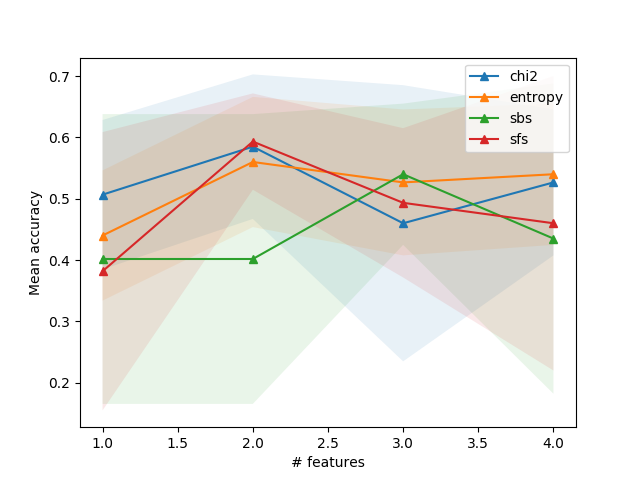
\includegraphics[width=\textwidth]{../plots_with_std_fill/ANNd1.png}
        \caption[]%
        {{\small}}
        \label{fig:ANN_MIAS}
    \end{subfigure}
    \hfill
    \begin{subfigure}[b]{0.7\textwidth}
        \centering
        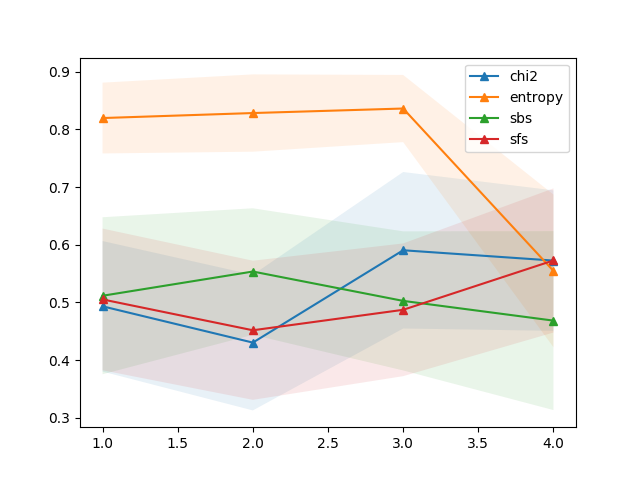
\includegraphics[width=\textwidth]{../plots_with_std_fill/ANNd2.png}
        \caption[]%
        {{\small}}
        \label{fig:ANN_EN}
    \end{subfigure}
    }
    \vskip
    \baselineskip
    \noindent\makebox[1.2\textwidth]{
    \begin{subfigure}[b]{0.7\textwidth}
        \centering
        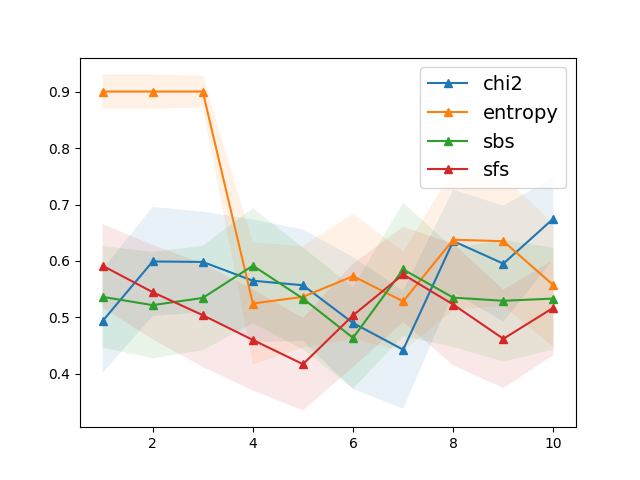
\includegraphics[width=\textwidth]{../plots_with_std_fill/ANNd3.png}
        \caption[]%
        {{\small}}
        \label{fig:ANN_RHH}
    \end{subfigure}
    \quad
    \begin{subfigure}[b]{0.7\textwidth}
        \centering
        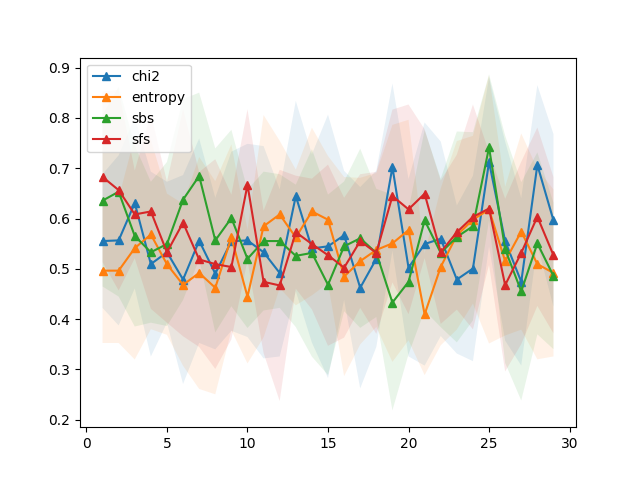
\includegraphics[width=\textwidth]{../plots_with_std_fill/ANNd4.png}
        \caption[]%
        {{\small}}
        \label{fig:ANN_WBCD}
    \end{subfigure}
    }

    \caption[]
    {\small
      Classifier ANN. Each plot corresponds to datasets (a) MIAS, (b) EN, (c) RHH and (d) WBCD. x-axis is number of features, y-axis is mean accuracy achieved by corresponding feature selection method. Shaded area represent the standard error for each FS-method.
    }
    \label{fig:plots_ANN}

\end{figure*}

\begin{figure*}[htbp]
  \noindent\makebox[1.1\textwidth]{
  \begin{subfigure}[b]{0.7\textwidth}
      \centering
      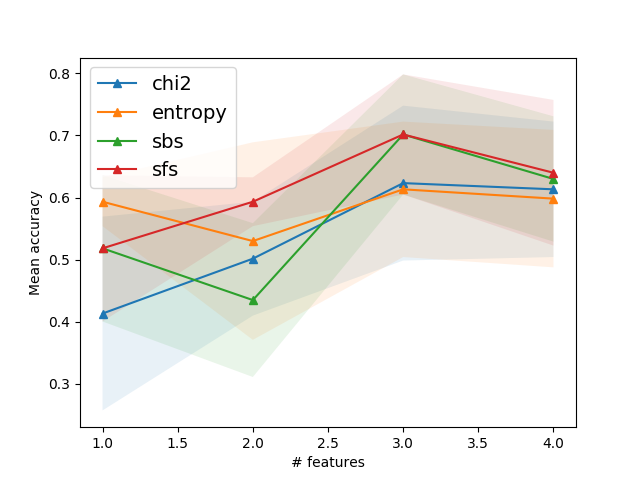
\includegraphics[width=\textwidth]{../plots_with_std_fill/CARTd1.png}
      \caption[]%
      {{\small}}
      \label{fig:CART_MIAS}
  \end{subfigure}
  \hfill
  \begin{subfigure}[b]{0.7\textwidth}
      \centering
      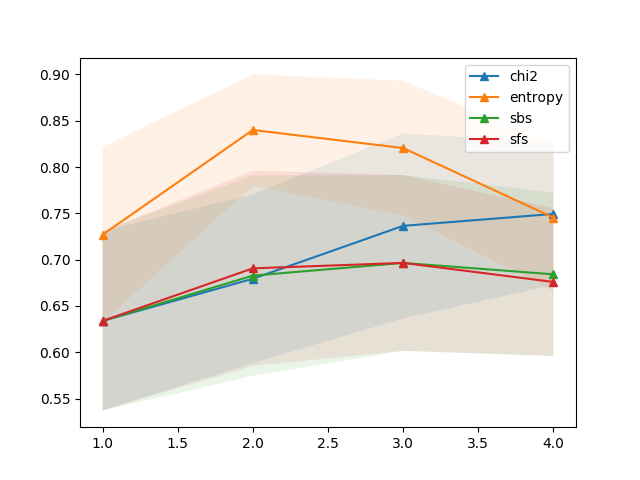
\includegraphics[width=\textwidth]{../plots_with_std_fill/CARTd2.png}
      \caption[]%
      {{\small}}
      \label{fig:CART_EN}
  \end{subfigure}

  }
  \vskip
  \baselineskip
  \noindent\makebox[1.1\textwidth]{

  \begin{subfigure}[b]{0.7\textwidth}
      \centering
      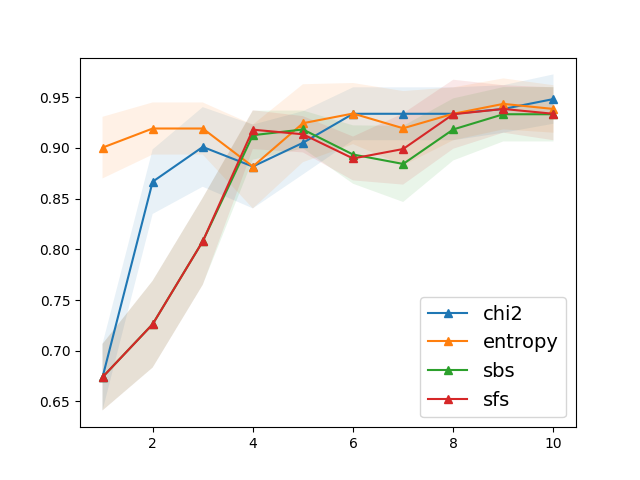
\includegraphics[width=\textwidth]{../plots_with_std_fill/CARTd3.png}
      \caption[]%
      {{\small}}
      \label{fig:CART_RHH}
  \end{subfigure}
  \hfill
  \begin{subfigure}[b]{0.7\textwidth}
      \centering
      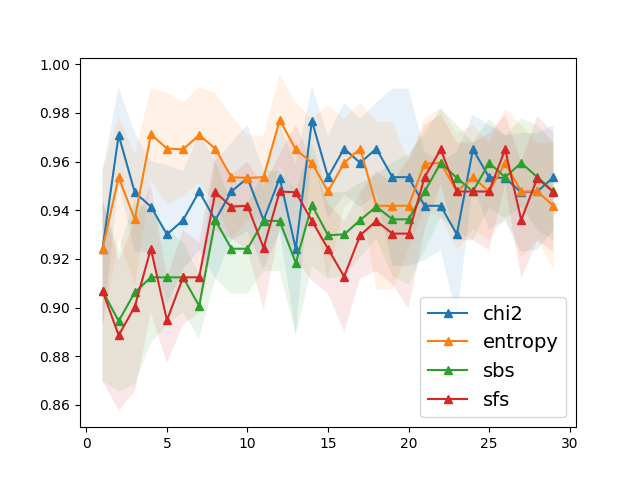
\includegraphics[width=\textwidth]{../plots_with_std_fill/CARTd4.png}
      \caption[]%
      {{\small}}
      \label{fig:CART_WBCD}
  \end{subfigure}
  }
  \caption[]
  {\small
    Classifier CART. Each plot corresponds to datasets (a) MIAS, (b) EN, (c) RHH and (d) WBCD. x-axis is number of features, y-axis is mean accuracy achieved by corresponding feature selection method. Shaded area represent the standard error for each FS-method.
  }
  \label{fig:plots_CART}
\end{figure*}

\begin{figure*}[htbp]
  \centering
  \begin{subfigure}[b]{0.475\textwidth}
      \centering
      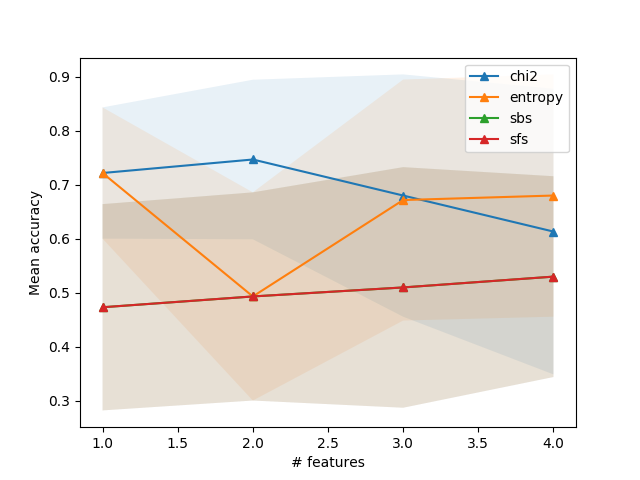
\includegraphics[width=\textwidth]{../plots_with_std_fill/NBd1.png}
      \caption[]%
      {{\small}}
      \label{fig:NB_MIAS}
  \end{subfigure}
  \hfill
  \begin{subfigure}[b]{0.475\textwidth}
      \centering
      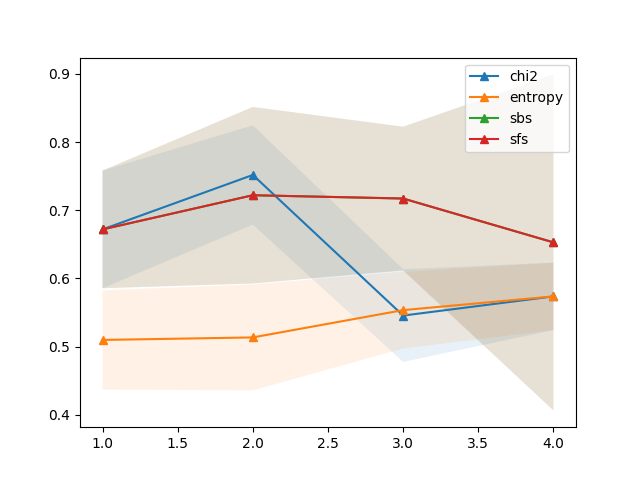
\includegraphics[width=\textwidth]{../plots_with_std_fill/NBd2.png}
      \caption[]%
      {{\small}}
      \label{fig:NB_EN}
  \end{subfigure}

  \begin{subfigure}[b]{0.475\textwidth}
      \centering
      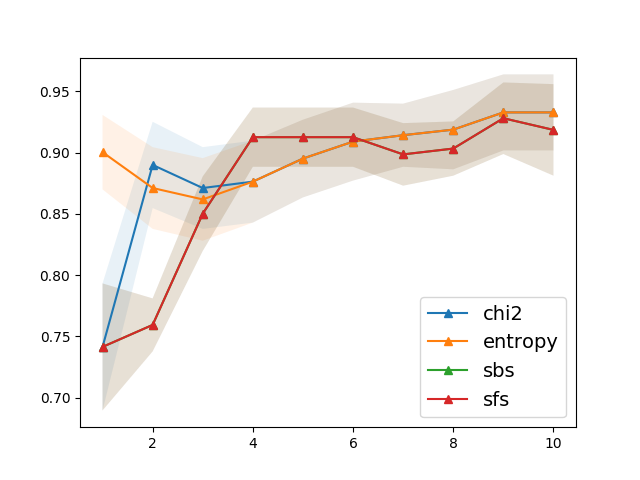
\includegraphics[width=\textwidth]{../plots_with_std_fill/NBd3.png}
      \caption[]%
      {{\small}}
      \label{fig:NB_RHH}
  \end{subfigure}
  \quad
  \begin{subfigure}[b]{0.475\textwidth}
      \centering
      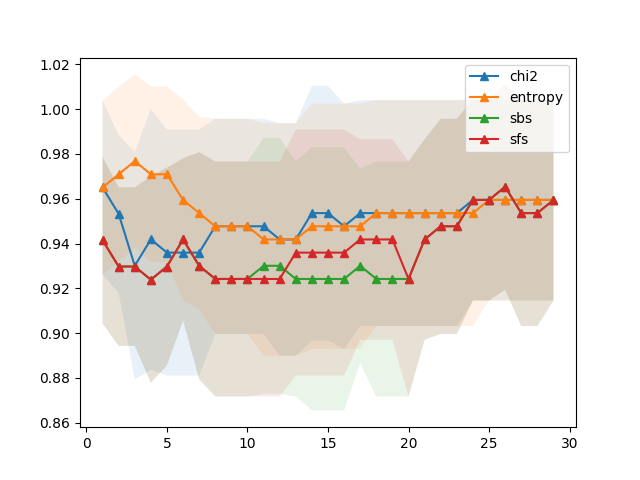
\includegraphics[width=\textwidth]{../plots_with_std_fill/NBd4.png}
      \caption[]%
      {{\small}}
      \label{fig:NB_WBCD}
  \end{subfigure}
  \caption[]
  {\small
    Classifier NB. Each plot corresponds to datasets (a) MIAS, (b) EN, (c) RHH and (d) WBCD. x-axis is number of features, y-axis is mean accuracy achieved by corresponding feature selection method.
  }
  \label{fig:plots_NB}
\end{figure*}

\begin{figure*}[htbp]
  \noindent\makebox[1.1\textwidth]{
  \begin{subfigure}[b]{0.7\textwidth}
      \centering
      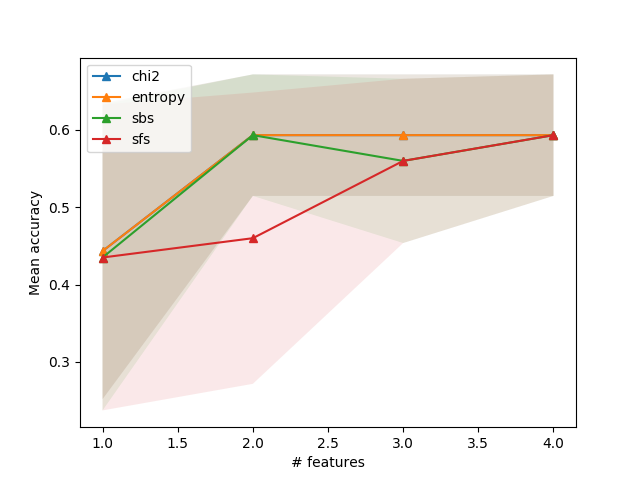
\includegraphics[width=\textwidth]{../plots_with_std_fill/SVMd1.png}
      \caption[]%
      {{\small}}
      \label{fig:SVM_MIAS}
  \end{subfigure}
  \hfill
  \begin{subfigure}[b]{0.7\textwidth}
      \centering
      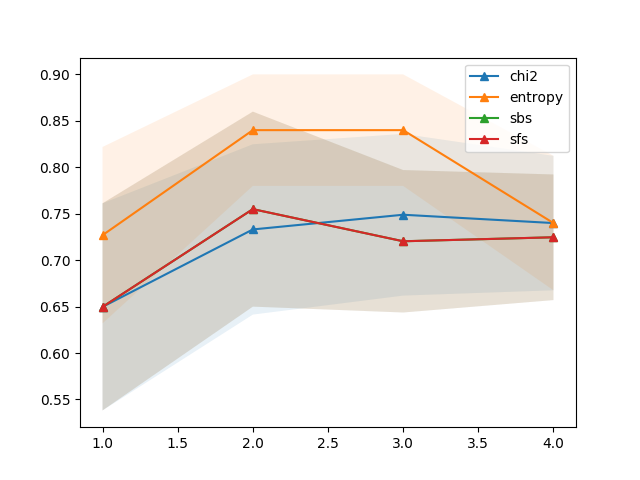
\includegraphics[width=\textwidth]{../plots_with_std_fill/SVMd2.png}
      \caption[]%
      {{\small}}
      \label{fig:SVM_EN}
  \end{subfigure}
  }
  \vskip
  \baselineskip
  \noindent\makebox[1.1\textwidth]{
  \begin{subfigure}[b]{0.7\textwidth}
      \centering
      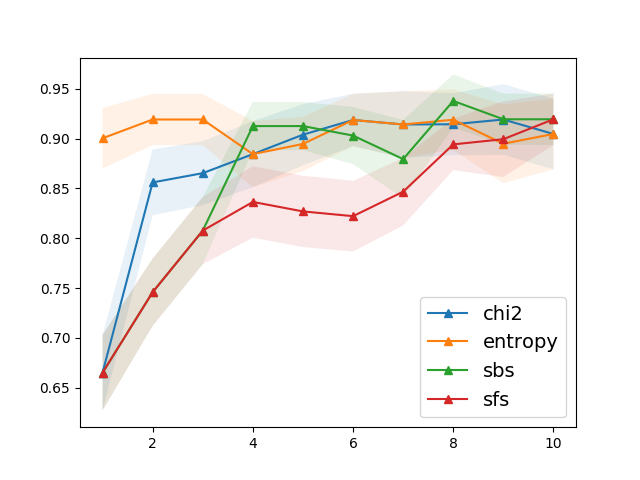
\includegraphics[width=\textwidth]{../plots_with_std_fill/SVMd3.png}
      \caption[]%
      {{\small}}
      \label{fig:SVM_RHH}
  \end{subfigure}
  \quad
  \begin{subfigure}[b]{0.7\textwidth}
      \centering
      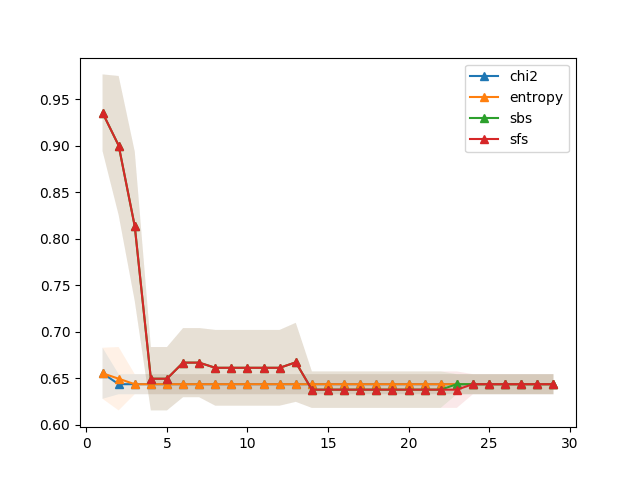
\includegraphics[width=\textwidth]{../plots_with_std_fill/SVMd4.png}
      \caption[]%
      {{\small}}
      \label{fig:SVM_WBCD}
  \end{subfigure}
  }
  \caption[]
  {\small
    Classifier SVM. Each plot corresponds to datasets (a) MIAS, (b) EN, (c) RHH and (d) WBCD. x-axis is number of features, y-axis is mean accuracy achieved by corresponding feature selection method. Shaded area represent the standard error for each FS-method.
  }
  \label{fig:plots_SVM}
\end{figure*}


\newpage
\section{Computation time}
\label{sec:cumtime}

Profiling the execution of running all experiments approximately 100\% of CPU-time was allocated to the Wrapper algorithms as showed in table \ref{table:cpu}. Finding the best possible subset of features is considered a NP-hard problem meaning a solution can not be found in polynomial time. This clearly suggest favouring filtering methods when choosing a feature selection method having limited computational resources.

\begin{table}[htbp]
\begin{center}
\begin{tabular}{|l|l|l|l|l|l|}
\cline{1-3}
\textbf{Function} & \textbf{Cumtime} & \textbf{Ratio}  \\
\cline{1-3}
          Chi2 &   3.759  &   0 \% \\
          Entropy &   42.8  &  0 \% \\
          SBS &   3751.879  &  15 \% \\
          SFS &   24785.653  & 87 \% \\

\cline{1-3}
\end{tabular}
\caption[]
{\small
  Table of CPU usage for the four FS methods. Cumtime is the cumulative time spent in this and all subfunctions (from invocation till exit). Ratio is the percentage of the total run time.
}
\label{table:cpu}
\end{center}
\end{table}




%
%
% ncalls  tottime  percall  cumtime  percall filename:lineno(function)
%
% 188    0.006    0.000   42.802    0.228 Main1_profile.py:103(entropyFunction)
%   1    0.005    0.005 28647.116 28647.116 Main1_profile.py:11(<module>)
% 188    0.002    0.000 24785.653  131.839 Main1_profile.py:111(sfsFunction)
% 188    0.003    0.000 3751.879   19.957 Main1_profile.py:119(sbsFunction)
% 752    0.033    0.000    0.045    0.000 Main1_profile.py:127(subsetFrom)
%  16    0.061    0.004 28646.085 1790.380 Main1_profile.py:131(evaluateMethod)
%   1    0.002    0.002 28646.236 28646.236 Main1_profile.py:35(main)
%   4    0.000    0.000    0.002    0.001 Main1_profile.py:92(splitData)
% 188    0.005    0.000    3.759    0.020 Main1_profile.py:95(chi2Function)

